% !TeX root = ../main.tex
% !TeX encoding = UTF-8
% !TeX spellcheck = none

\section{方法学}\label{sec:methodology}

\subsection{总体框架}\label{sec:framework}

CMSRN 的整体架构如图~\ref{fig:cmsrn-architecture}所示。框架首先通过共享双频时空编码形成基础预测；SERR 利用自身演化与有向时滞两类专家组织修正证据，BCMS 根据双端流量背景与预测时距选择跨区域历史消息。两个模块分别读取共享表征、生成互补修正，并在预测端进行加性融合：
\begin{equation}
\label{eq:overall-prediction}
\widetilde{Y}=\widetilde{Y}^{0}+\Delta\widetilde{Y}^{S}+\Delta\widetilde{Y}^{B}.
\end{equation}
其中，\(\widetilde{Y}^{0}\)为基础预测，\(\Delta\widetilde{Y}^{S}\)和\(\Delta\widetilde{Y}^{B}\)分别为 SERR 与 BCMS 的修正，三者均属于\(\mathbb{R}^{H\times N\times2}\)。波浪号表示按流量通道标准化的预测量。下文将历史窗口内的位置重编号为\(k=1,\ldots,T\)，未来预测步记为\(h=1,\ldots,H\)，并用\(c\in\{\mathrm{in},\mathrm{out}\}\)区分流量通道。

\begin{figure}[!htbp]
  \centering
  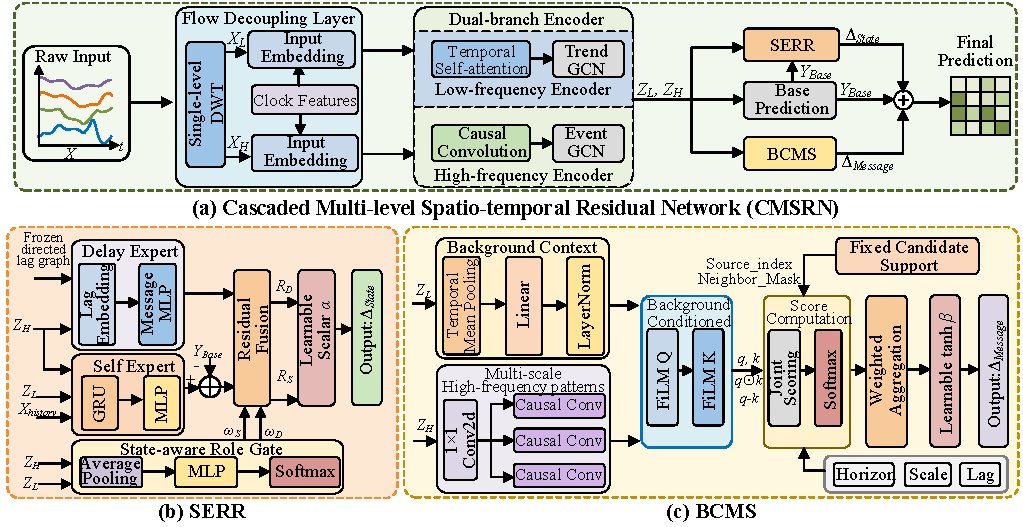
\includegraphics[width=\linewidth]{figures/model-architecture.pdf}
  \caption[CMSRN 的整体架构]{\textbf{CMSRN 的整体架构及核心模块。}（a）历史流量经单层小波分解与双分支时空编码形成低、高频表征，基础预测与 SERR、BCMS 产生的修正量在预测端融合。（b）SERR 通过自身演化专家、有向时滞专家及状态感知角色门控，生成角色相关的残差修正。（c）BCMS 利用低频背景调制高频多尺度模式匹配，针对不同预测步，对固定候选邻域内的邻居--时滞--尺度组合进行联合评分与加权聚合。图中的\(Y_{\mathrm{Base}}\)、\(\Delta\mathrm{State}\)和\(\Delta\mathrm{Message}\)分别对应\(\widetilde{Y}^{0}\)、\(\Delta\widetilde{Y}^{S}\)和\(\Delta\widetilde{Y}^{B}\)，均在标准化流量尺度下表示。}
  \label{fig:cmsrn-architecture}
\end{figure}

\subsection{共享双频时空表征}\label{sec:dual-frequency}

为区分平缓变化与短时波动，CMSRN 采用 TEDDCF~\cite{ref18}的低、高频双分支结构提取共享表征。首先，沿历史窗口的时间维对各流量通道进行单层离散小波分解与重构，得到低频和高频序列。两类序列均使用训练期流量的逐通道均值与标准差进行标准化，再附加日内时刻与星期信息，形成\(U_L,U_H\in\mathbb{R}^{T\times N\times4}\)。两分支共享输入投影与时间嵌入，随后分别执行低频时间自注意力及趋势图编码、高频时间卷积及事件图编码：
\begin{equation}
\label{eq:low-frequency}
Z_L=\mathrm{F}_L(U_L),
\end{equation}
\begin{equation}
\label{eq:high-frequency}
Z_H=\mathrm{F}_H(U_H),
\end{equation}
其中，\(Z_L,Z_H\in\mathbb{R}^{T\times N\times d_b}\)，\(d_b\)为共享表征维度。基础预测由两类特征融合后获得：
\begin{equation}
\label{eq:base-prediction}
\widetilde{Y}^{0}=\mathrm{R}\!\left(\operatorname{ReLU}\!\left[Z_L+\operatorname{GLU}(Z_L)+Z_H\right]\right).
\end{equation}
\(\mathrm{R}\)为覆盖完整历史窗口的卷积预测头，将特征映射为未来\(H\)步的流入与流出预测。SERR 和 BCMS 使用的\(Z_L\)取自 GLU 之前，与\(Z_H\)共同作为共享输入。

\subsection{状态证据驱动的异质角色残差精炼}\label{sec:serr}

SERR 按照节点自身演化与跨区域时滞关联组织两类互补专家，并根据当前状态分配其修正贡献，如图~\ref{fig:cmsrn-architecture}（b）所示。为连接常规参照与近期动态，记\(x_{k,i,c}\)为历史位置\(k\)处节点\(i\)的通道\(c\)原始流量，\(b_{k,i,c}\)为对应的训练期常规基线。状态证据定义为：
\begin{equation}
\label{eq:state-evidence}
\begin{aligned}
\bar{x}_{k,i,c}&=\frac{1}{\ell_k}\sum_{r=k-\ell_k+1}^{k}x_{r,i,c},\qquad \ell_k=\min(3,k),\\
e_{i,c}&=\left[\bar{x}_{T,i,c}-b_{T,i,c},\;x_{T,i,c}-\bar{x}_{T,i,c}\right]^{\mathsf T}.
\end{aligned}
\end{equation}
\(e_{i,c}\in\mathbb{R}^{2}\)分别描述末时刻的趋势偏差与短时波动。均值仅使用当前历史窗口内已观测的位置，窗口起始处按可用长度计算。

自身演化专家在各节点内编码近期轨迹。对于每个流量通道，将共享双频特征之和与原始流量拼接，输入共享 GRU，并将末隐藏状态映射为多步预测：
\begin{equation}
\label{eq:self-expert}
P^{\mathrm{self}}_{:,i,c}
=\mathcal{P}_{S}\!\left(\psi_S\!\left(\operatorname{GRU}_{\mathrm{last}}
\left([Z_{L,k,i}+Z_{H,k,i}\,\Vert\,x_{k,i,c}]_{k=1}^{T}\right)\right)\right).
\end{equation}
其中，\(\Vert\)表示特征拼接，\(\psi_S\)为含 Tanh 激活的两层感知机，\(\mathcal{P}_S\)将\(d_b\)维特征线性映射为\(H\)步预测。该分支在共享时空表征上进一步提取节点自身的时间演化信息。

有向时滞专家从预先构建并冻结的关系集合\(\mathcal{E}_c\)中提取来源节点历史特征。对边\((j,i,\ell)\in\mathcal{E}_c\)，\(j\)为来源节点，\(i\)为目标节点，\(\ell\)为满足\(0<\ell<T\)的历史时滞。来源高频特征经滞后嵌入调制，并结合目标状态证据转换为补充消息：
\begin{equation}
\label{eq:delay-expert}
\begin{aligned}
\eta_{i,c}&=W_e e_{i,c},\\
m_{j\to i,\ell,c}&=\psi_D\!\left([(1+\tanh v_{\ell})\odot Z_{H,T-\ell,j}\,\Vert\,\eta_{i,c}]\right),\\
R^{\mathrm{delay}}_{:,i,c}&=\mathcal{P}_D\!\left(\eta_{i,c}
+\sum_{(j,i,\ell)\in\mathcal{E}_c}a_{ji\ell}^{c}m_{j\to i,\ell,c}\right).
\end{aligned}
\end{equation}
这里，\(W_e\in\mathbb{R}^{d_b\times2}\)为证据投影，\(v_\ell\in\mathbb{R}^{d_b}\)为可学习滞后嵌入，\(\psi_D\)为含 SiLU 激活的无偏置消息变换，\(a_{ji\ell}^{c}\)为固定边权，\(\mathcal{P}_D\)为多步线性输出头。两类专家各自的参数在节点和流量通道间共享，有向时滞关系按流量通道分别给定。

状态条件门控利用低、高频特征的时间均值及两类流量的状态证据，确定专家贡献：
\begin{equation}
\label{eq:role-gate}
\Omega_i=\operatorname{Softmax}_{\mathrm{expert}}\!\left(
\operatorname{reshape}_{2\times2}\,g\!\left(
[\bar{Z}_{L,i}\,\Vert\,\bar{Z}_{H,i}\,\Vert\,e_{i,\mathrm{in}}\,\Vert\,e_{i,\mathrm{out}}]
\right)\right).
\end{equation}
\(\bar{Z}_{L,i},\bar{Z}_{H,i}\)为沿历史时间维求均值得到的\(d_b\)维向量，\(g\)为含 SiLU 激活的两层感知机。\(\Omega_i\in\mathbb{R}^{2\times2}\)的行对应流量通道，列对应自身与时滞专家，Softmax 在专家维归一化，得到\(\omega^S_{i,c}\)和\(\omega^D_{i,c}\)。这些权重随样本、节点与流量通道变化，并在全部预测步间共享。最终修正为：
\begin{equation}
\label{eq:serr-residual}
\Delta\widetilde{Y}^{S}_{h,i,c}
=\alpha\left[\omega^S_{i,c}\left(P^{\mathrm{self}}_{h,i,c}-\widetilde{Y}^{0}_{h,i,c}\right)
+\omega^D_{i,c}R^{\mathrm{delay}}_{h,i,c}\right].
\end{equation}
\(P^{\mathrm{self}}\)与\(R^{\mathrm{delay}}\)均对应基础预测所在的标准化流量尺度，\(\alpha\)为全局可学习标量。自身专家通过相对于基础预测的残差参与修正，时滞专家则提供跨区域历史信息的补偿，两者由状态条件门控协同融合。

\subsection{背景条件化的联合历史消息选择}\label{sec:bcms}

BCMS 在固定候选邻域内，依据当前背景及未来预测时距选择历史消息，如图~\ref{fig:cmsrn-architecture}（c）所示。首先，将低频特征的时间均值映射为节点背景，并对高频特征提取多尺度模式：
\begin{equation}
\label{eq:bcms-context-pattern}
\xi_i=\operatorname{LN}\!\left(\mathcal{P}_b(\bar{Z}_{L,i})\right),
\qquad z^s=\mathcal{T}_s\!\left(\mathcal{P}_H(Z_H)\right).
\end{equation}
\(\xi_i\in\mathbb{R}^{d}\)，\(z^s\in\mathbb{R}^{T\times N\times d}\)，其中\(d=32\)。\(\mathcal{P}_b\)为线性投影，\(\mathcal{P}_H\)为各尺度共享的\(1\times1\)卷积。\(\mathcal{T}_s\)由左侧填充的深度时间卷积、逐点卷积和 GELU 构成；三个尺度采用大小为3的卷积核及扩张率1、2、4，对应时间覆盖范围\(r_s\in\{3,5,9\}\)。

记节点\(i\)的固定候选来源集合为\(\mathcal{N}_i\)，历史时滞\(\tau\in\{0,1,2,3\}\)。有效候选集合为\(\mathcal{A}_i=\{(j,\tau,s):j\in\mathcal{N}_i,\ r_s+\tau\leq T\}\)，其中每个节点至多保留8个来源。对同一尺度上的目标末时刻模式与来源历史模式，分别使用双端低频背景调制查询和键：
\begin{equation}
\label{eq:background-conditioned-qk}
\begin{aligned}
q_i^s&=(1+\gamma_q(\xi_i))\odot Q(z^s_{T,i})+\delta_q(\xi_i),\\
k_{j,\tau}^s&=(1+\gamma_k(\xi_j))\odot K(z^s_{T-\tau,j})+\delta_k(\xi_j).
\end{aligned}
\end{equation}
\(Q,K\)为可学习仿射映射，\(\gamma\)和\(\delta\)分别产生\(d\)维缩放与平移参数。由此，高频模式的匹配同时受目标与来源区域的低频背景约束。

对于预测步\(h\)，联合评分定义为：
\begin{equation}
\label{eq:joint-message-score}
\begin{aligned}
u_{i,j,\tau,s}
&=A_q q_i^s+A_k k_{j,\tau}^s
+A_p(q_i^s\odot k_{j,\tau}^s)+A_d(q_i^s-k_{j,\tau}^s)+b_a,\\
a_{h,i,j,\tau,s}
&=w_a^{\mathsf T}\operatorname{GELU}\!\left(
u_{i,j,\tau,s}+e_{\mathrm{lag}}(\tau)+e_{\mathrm{scale}}(r_s)+e_{\mathrm{hor}}(h)\right).
\end{aligned}
\end{equation}
其中，\(A_q,A_k,A_p,A_d\in\mathbb{R}^{d\times d}\)，\(b_a,w_a\in\mathbb{R}^{d}\)为可学习参数。三类时间编码分别对\([v,\sin(2\pi v),\cos(2\pi v)]^{\mathsf T}\)进行无偏置线性投影，\(v\)为相应时滞、尺度覆盖范围或预测时距换算得到的小时数。预测步编码在非线性评分之前引入，使候选贡献随未来时距变化。

为调节历史信息的总体引入程度，在每个预测步的候选集合中加入分数和值均为零的消息选项。对真实候选，联合归一化权重为：
\begin{equation}
\label{eq:joint-message-softmax}
w_{h,i,j,\tau,s}
=\frac{\exp(a_{h,i,j,\tau,s})}
{1+\displaystyle\sum_{(j',\tau',s')\in\mathcal{A}_i}\exp(a_{h,i,j',\tau',s'})}.
\end{equation}
分母中的1对应零消息，其占据的概率质量允许降低真实历史消息的总权重。来源高频模式经值投影后加权聚合，并生成双通道修正：
\begin{equation}
\label{eq:bcms-residual}
\begin{aligned}
m_{h,i}&=\sum_{(j,\tau,s)\in\mathcal{A}_i}
w_{h,i,j,\tau,s}W_vz^s_{T-\tau,j},\\
\Delta\widetilde{Y}^{B}_{h,i,:}&=\tanh(\beta)\,W_o m_{h,i}.
\end{aligned}
\end{equation}
\(W_v\in\mathbb{R}^{d\times d}\)与\(W_o\in\mathbb{R}^{2\times d}\)均为无偏置投影，\(\beta\)为全局可学习标量。流入与流出共享消息选择权重和聚合表示，由双输出头形成对应修正。BCMS 的权重针对每个预测步生成，与 SERR 在预测步间共享的专家权重形成互补。

\subsection{联合预测输出}\label{sec:joint-output}

将两类修正按式~\eqref{eq:overall-prediction}叠加至基础预测后，使用训练期输入窗口估计并固定的逐通道统计量恢复原始流量尺度：
\begin{equation}
\label{eq:inverse-scaling}
\widehat{Y}_{t+h,i,c}
=\sigma_c\left(\widetilde{Y}^{0}_{h,i,c}
+\Delta\widetilde{Y}^{S}_{h,i,c}+\Delta\widetilde{Y}^{B}_{h,i,c}\right)+\mu_c.
\end{equation}
其中，\(\mu_c\)和\(\sigma_c\)分别为通道\(c\)的均值与标准差。两个全局强度参数\(\alpha\)和\(\beta\)均初始化为零，因此初始输出与基础预测一致；SERR 门控末层同时采用零初始化，使两类专家初始权重均为0.5。模型由此在统一的流入与流出预测目标下学习两条互补修正通路的贡献。
